% 依试点教材理科固定来源 PDF 第 2 页转绘梯形与棱锥的拓扑关系；不表示精确比例。
\begin{center}
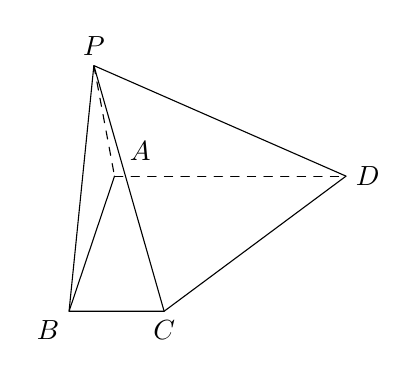
\begin{tikzpicture}[x=1.05cm,y=0.78cm,>=stealth,line cap=round,line join=round]
  \coordinate (B) at (0,0);
  \coordinate (A) at (0.55,2.2);
  \coordinate (C) at (1.15,0);
  \coordinate (D) at (3.35,2.2);
  \coordinate (P) at (0.3,4.0);
  \draw (A)--(B)--(C)--(D);
  \draw[dashed] (A)--(D);
  \draw (P)--(B) (P)--(C) (P)--(D);
  \draw[dashed] (P)--(A);
  \node[above right,xshift=2pt,yshift=2pt] at (A) {$A$};
  \node[below left] at (B) {$B$};
  \node[below] at (C) {$C$};
  \node[right] at (D) {$D$};
  \node[above] at (P) {$P$};
\end{tikzpicture}
\end{center}
